\section{Results}
\label{sec:results}

\subsection{Main results}
\cref{fig:main_results} compares the performance achieved by our method against that of the different fixed strategies and the estimated best fixed strategy when using $\alpha_s = 12$ across the different datasets. From these results we can make a number of key observations. 
%\begin{figure*}[h]
%\centering
%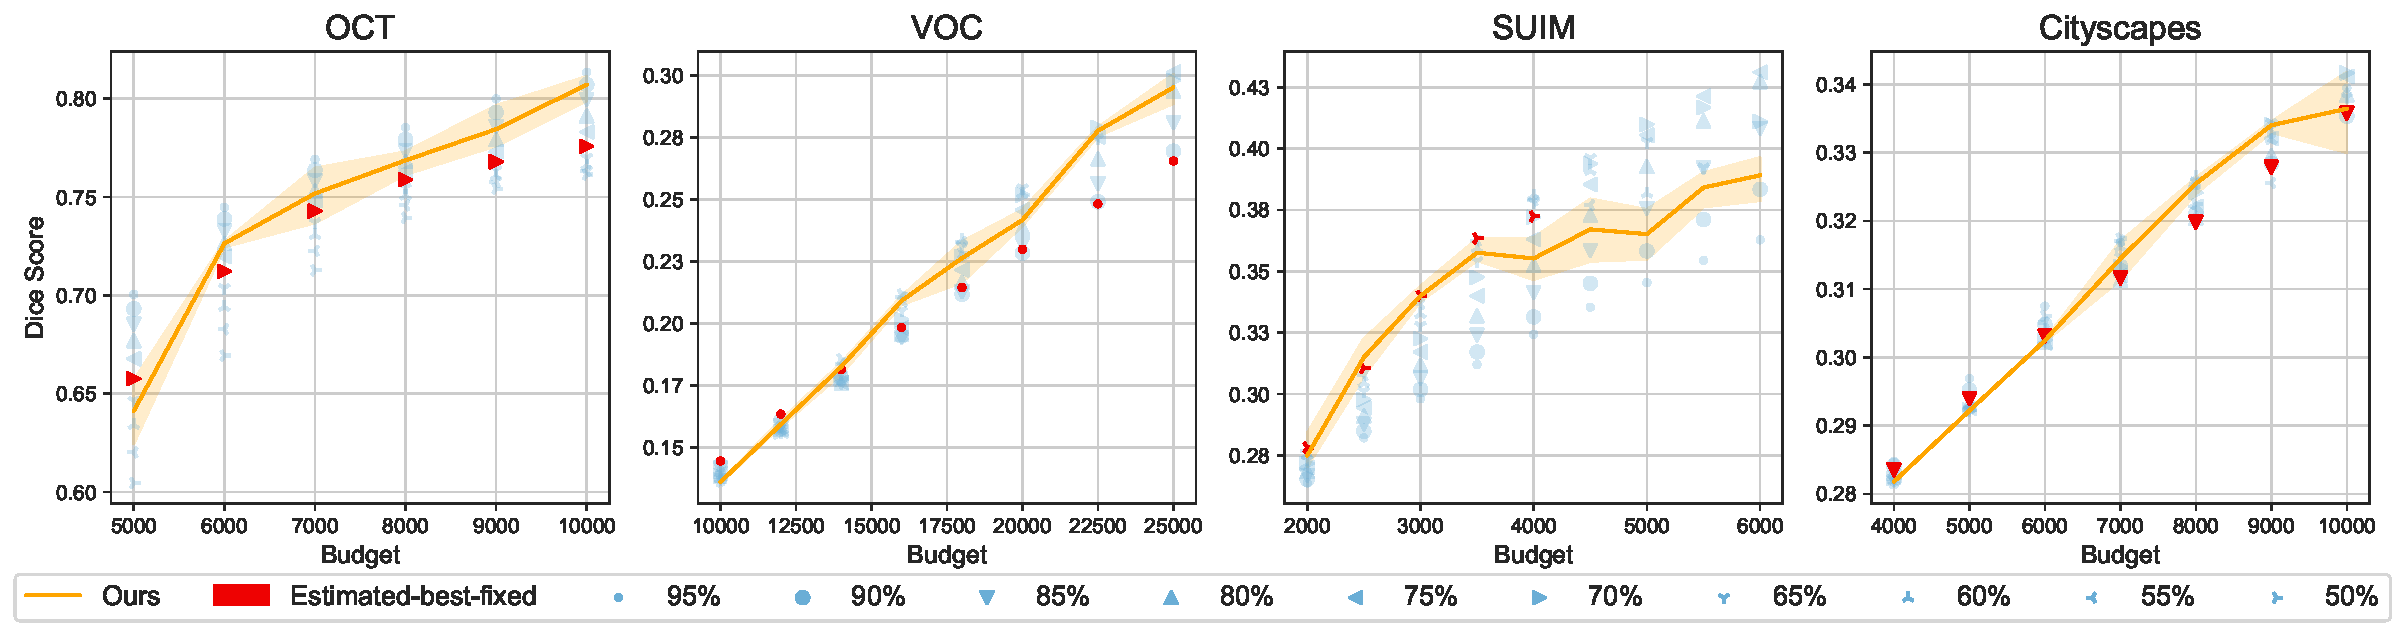
\includegraphics[width=\textwidth]{Figures/main_result_notshared.pdf}
%\caption{
%Performance of our method (orange line) on OCT, PASCAL VOC, SUIM and Cityscapes datasets. Shaded region is computed from three seeds. Fixed strategies are shown in blue. Red points show the {\it estimated-best-fixed} strategy with $B_0$.  Labels expressed as percentage of the budget allocated to segmentation. Note that the first budget $B$ fulfills $B\gg B_0$ in all cases. 
%}
%\label{fig:main_results}
%\end{figure*}
\plainwidefig{1}{Figures/main_result_notshared.pdf}{Performance of our method (orange line) on OCT, PASCAL VOC, SUIM and Cityscapes datasets. Shaded region is computed from three seeds. Fixed strategies are shown in blue. Red points show the \textit{estimated-best-fixed} strategy with $B_0$. Labels expressed as percentage of the budget allocated to segmentation. Note that the first budget $B$ fulfills $B\gg B_0$ in all cases.}{fig:main_results}

First, we can observe that no single fixed strategy is performing optimally across the different datasets evaluated. This is coherent with our initial claims and with the literature. Indeed, for OCT the best strategy appears to be one that samples 90\% of segmentations, while this same policy performs poorly on the SUIM dataset. This implies that blindly using a fixed policy would on average not be very effective.

Second, the estimated best-fixed strategy (in red) appears to do well initially and progressively loses competitiveness as the budget increases. This behaviour is expected as the estimated fixed strategy is that with $B_0$ (the lowest budget), and becomes increasingly irrelevant as $B$ grows. This is particularly clear on VOC where the best low-budget strategy allocates 95\% of the budget to segmentation and still achieves superior performance up to $B=12'000$. However, that strategy drops below average performance with budgets greater than $B=25'000$. In the case of SUIM, the best-fixed strategy corresponds to 50\% of the budget allocated to segmentation. Since the dataset contains only 1'525 segmentation samples, this strategy is not attainable with $B > 4'000$.

Last, we can observe that our method is consistently able to produce good performances, across both different budget quantities and datasets. We can also clearly see that our strategy is not guaranteed to be the top performing strategy, but that on average it performs well in different cases. 

At the same time, we notice that the performance of our approach on SUIM begins well and then drops after a 3'500 budget. This differs sharply from the other datasets. By observing the true budget-performance surface of SUIM and the other datasets (see \cref{fig:surfaces}), we can see that the SUIM surface does not grow logarithmically with the dataset size, while it does for Cityscapes (and the other too, see the Supplementary materials). This is relevant as our GP mean prior~\eqref{eq:gp_mean} assumes this relationship and explains why our approach fails when the true surface deviates from our GP mean form. While the use of adaptive, higher-level order priors would be beneficial to deal with such cases, we leave this as future work to be researched.

\marginfig{Figures/surfaces.pdf}{Cityscapes (top) and SUIM (bottom) ground truth budget-segmentation surfaces. We note that segmentation performance grows logarithmically with training set size on Cityscapes (as well as OCT and VOC, see \Cref{fig:surfaces_fullweak_app} in the Appendix). This trend is not observed in the SUIM dataset.}{fig:surfaces}


\subsection{Sensitivity to $\alpha_s$ and $T$}
Different types of annotations or domains may have different ratios of cost. While we have fixed $\alpha_s$ in our experiments across all datasets regardless of their domain, some datasets such as OCT and VOC require different expertise and domain knowledge to annotate and thus different $\alpha_s$. In~\cref{fig:alpha_results}, we three additional values of $\alpha_s = \{5, 12, 25, 50\}$ and show the performance implication it has on our methods and the baselines. For Cityscapes, we see that the method is robust regardless of the value of $\alpha_s$, showing above average performance, especially for $\alpha_s = 25$ and $\alpha_s = 50$. This behavior is reproduced in all four datasets, as shown in \Cref{fig:surfaces_fullweak_app} in the Appendix.

\plainwidefig[b]{1}{Figures/alphas_notshared.pdf}{Mean of our method with $\alpha_s = \{5, 12, 25, 50\}$ on Cityscapes (orange, line). Shaded region is computed from three seeds. Fixed strategies are shown in blue. Labels expressed as percentage of the budget allocated to segmentation.}{fig:alpha_results}

%\begin{figure}[]
%\centering
%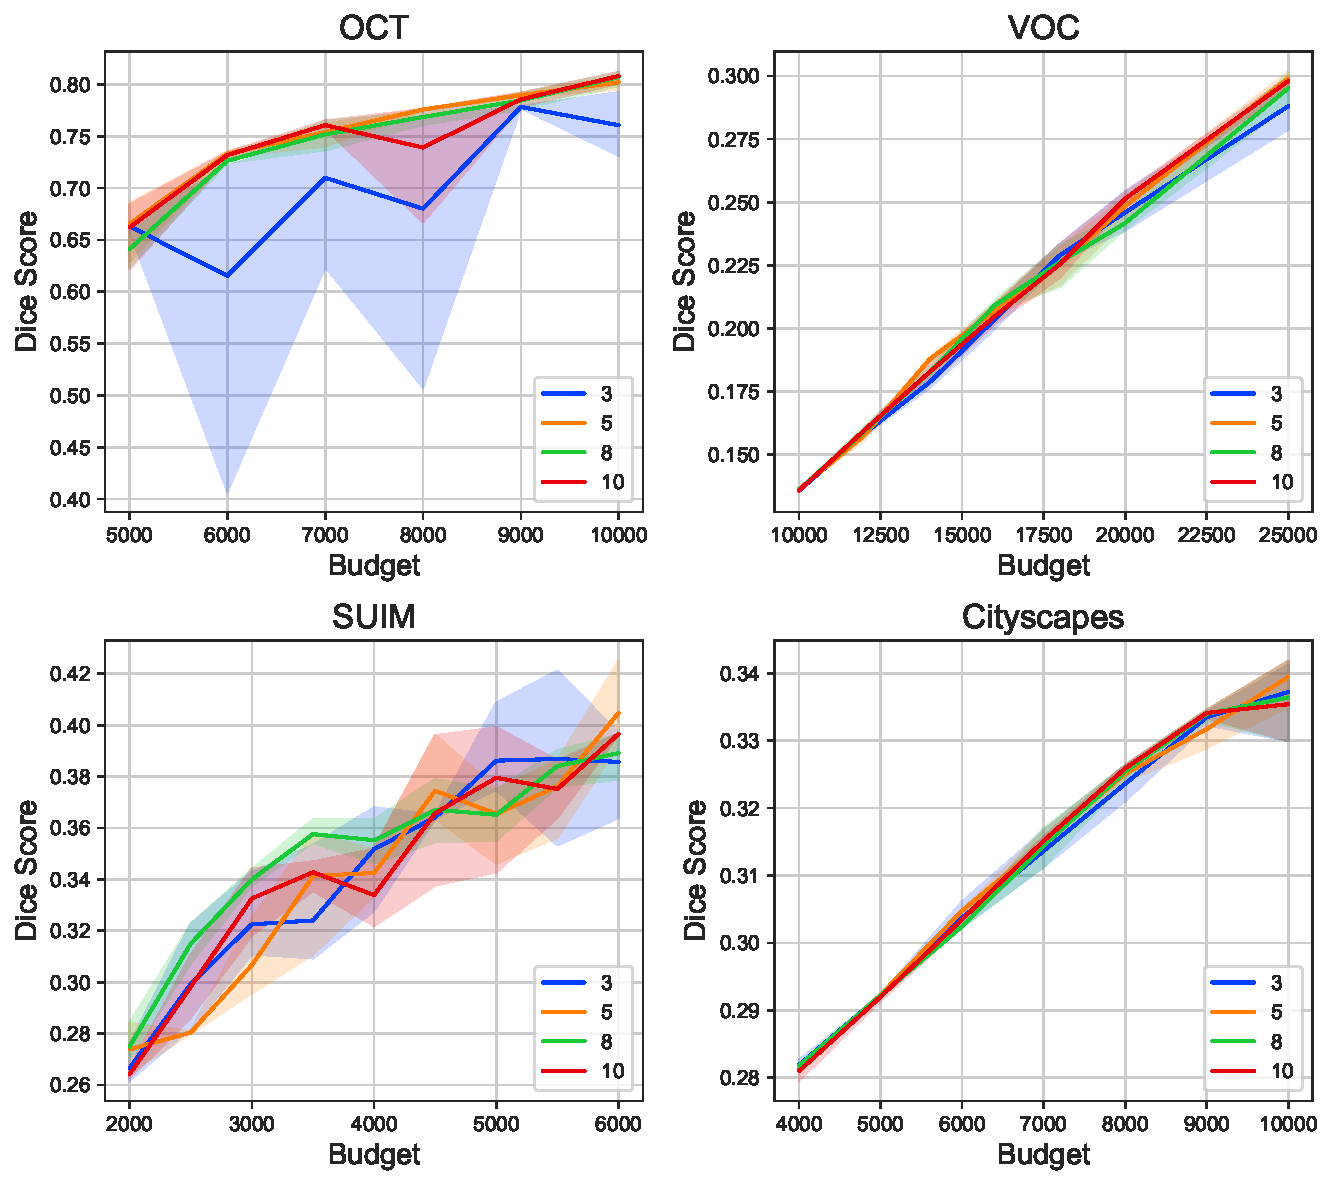
\includegraphics[width=0.8\linewidth]{Figures/steps_notshared_square.pdf}
%\caption{Mean of our method when using different numbers of iteration steps $\{3, 5, 8, 10\}$. Results shown with three seeds.
%}
%\label{fig:steps_results}
%\end{figure}

Similarly, the number of steps $T$ given to reach the final budget is a hyperparameter of our approach. While low $T$ values could lead to poor solutions due to the unreliability of the GP far from the sampled region, higher $T$ values\sidenote{And therefore smaller steps.} may exacerbate the intrinsic greedy nature of our method. We thus seek a trade-off between reliability and greediness. To study the sensitivity of the algorithm with respect to this variable, we show the behaviour of our method with different number of steps in~\cref{fig:steps_results}. We see that lower $T$ values greatly affect the reliability of the found strategy, especially for OCT and SUIM (blue line). However, as the number of steps increases, the variance of the strategy reduces sharply. We can therefore conclude that the method is robust to this hyperparameter as long as it is kept within reasonable ranges.

\textfig[h]{1}{Figures/steps_notshared_square.pdf}{Mean of our method when using different numbers of iteration steps $\{3, 5, 8, 10\}$. Results shown with three seeds.}{fig:steps_results}